\section{Register description}
\regover{
{\hyperref[dsi-dsi-config]{dsi\_config}}&
\\
\hline
{\hyperref[dsi-dsi-esc-config]{dsi\_esc\_config}}&
\\
\hline
{\hyperref[dsi-dsi-lpdt-tx-config]{dsi\_lpdt\_tx\_config}}&
\\
\hline
{\hyperref[dsi-dsi-hstx-config]{dsi\_hstx\_config}}&
\\
\hline
{\hyperref[dsi-dsi-int-status]{dsi\_int\_status}}&
\\
\hline
{\hyperref[dsi-dsi-int-mask]{dsi\_int\_mask}}&
\\
\hline
{\hyperref[dsi-dsi-int-clear]{dsi\_int\_clear}}&
\\
\hline
{\hyperref[dsi-dsi-int-enable]{dsi\_int\_enable}}&
\\
\hline
{\hyperref[dsi-dsi-fifo-config-0]{dsi\_fifo\_config\_0}}&
\\
\hline
{\hyperref[dsi-dsi-fifo-config-1]{dsi\_fifo\_config\_1}}&
\\
\hline
{\hyperref[dsi-dsi-fifo-wdata]{dsi\_fifo\_wdata}}&
\\
\hline
{\hyperref[dsi-dsi-fifo-rdata]{dsi\_fifo\_rdata}}&
\\
\hline
{\hyperref[dsi-dphy-config-0]{dphy\_config\_0}}&
\\
\hline
{\hyperref[dsi-dphy-config-1]{dphy\_config\_1}}&
\\
\hline
{\hyperref[dsi-dphy-config-2]{dphy\_config\_2}}&
\\
\hline
{\hyperref[dsi-dphy-config-3]{dphy\_config\_3}}&
\\
\hline
{\hyperref[dsi-dphy-config-4]{dphy\_config\_4}}&
\\
\hline
{\hyperref[dsi-dphy-config-5]{dphy\_config\_5}}&
\\
\hline
{\hyperref[dsi-dphy-config-6]{dphy\_config\_6}}&
\\
\hline
{\hyperref[dsi-dphy-config-7]{dphy\_config\_7}}&
\\
\hline
{\hyperref[dsi-dphy-config-8]{dphy\_config\_8}}&
\\
\hline
{\hyperref[dsi-dphy-config-9]{dphy\_config\_9}}&
\\
\hline
{\hyperref[dsi-dphy-config-10]{dphy\_config\_10}}&
\\
\hline
{\hyperref[dsi-dphy-config-11]{dphy\_config\_11}}&
\\
\hline
{\hyperref[dsi-dphy-config-12]{dphy\_config\_12}}&
\\
\hline
{\hyperref[dsi-dphy-config-13]{dphy\_config\_13}}&
\\
\hline
{\hyperref[dsi-dphy-config-14]{dphy\_config\_14}}&
\\
\hline
{\hyperref[dsi-dphy-config-15]{dphy\_config\_15}}&
\\
\hline
{\hyperref[dsi-dphy-config-16]{dphy\_config\_16}}&
\\
\hline
{\hyperref[dsi-dummy-reg]{dummy\_reg}}&
\\
\hline
}

\subsection{dsi\_config}
\label{dsi-dsi-config}
Address:0x3001a100
 \begin{figure}[H]
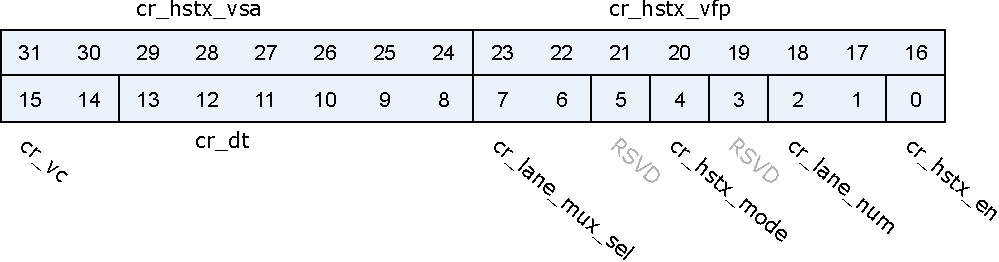
\includegraphics{dsi_dsi_config.pdf}
\end{figure}

\regdes{31:24&cr\_hstx\_vsa&r/w&8'd2&HSTX Vertical Sync Active width\\\hline
23:16&cr\_hstx\_vfp&r/w&8'd2&HSTX Vertical Front Porch width\\\hline
15:14&cr\_vc&r/w&2'd0&Virtual Channel number\\\hline
13:8&cr\_dt&r/w&6'h3E&Data Type \par 6'h2C: YUV422, 8-bit \par 6'h0E: RGB565 \par 6'h2E: RGB666, loosely packed \par 6'h3E: RGB888 \par Others: Reserved
\\\hline
7:6&cr\_lane\_mux\_sel&r/w&2'd0&Controls lane order \par 2'd0: {lane3, lane2, lane1, lane0} (no lane is switched) \par 2'd1: {lane2, lane1, lane3, lane0} \par 2'd2: {lane1, lane3, lane2, lane0} \par 2'd3: {lane3, lane1, lane2, lane0}
\\\hline
5&RSVD& & & \\\hline
4&cr\_hstx\_mode&r/w&1'b1&HSTX mode select \par 1'b0: Sync Event mode \par 1'b1: Sync Pulse mode
\\\hline
3&RSVD& & & \\\hline
2:1&cr\_lane\_num&r/w&2'd0&Lane number configuration \par 2'd0: 1-lane MIPI TX \par 2'd1: 2-lane MIPI TX \par 2'd2: 4-lane MIPI TX \par 2'd3: Reserved
\\\hline
0&cr\_hstx\_en&r/w&1'b0&HSTX function enable signal\\\hline

}
\subsection{dsi\_esc\_config}
\label{dsi-dsi-esc-config}
Address:0x3001a104
 \begin{figure}[H]
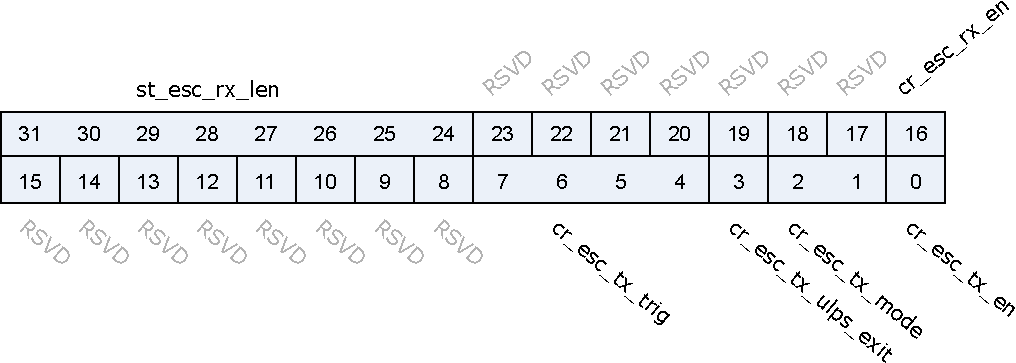
\includegraphics{dsi_dsi_esc_config.pdf}
\end{figure}

\regdes{31:24&st\_esc\_rx\_len&r&8'd0&Escape RX length received (Include packet header/data/footer) (unit: byte)\\\hline
23:17&RSVD& & & \\\hline
16&cr\_esc\_rx\_en&r/w&1'b0&Escape RX enable signal\\\hline
15:8&RSVD& & & \\\hline
7:4&cr\_esc\_tx\_trig&r/w&4'h0&Escape TX trigger command\\\hline
3&cr\_esc\_tx\_ulps\_exit&w1p&1'b0&Escape TX ULPS exit signal trigger\\\hline
2:1&cr\_esc\_tx\_mode&r/w&2'd0&Escape TX mode select \par 2'd0: LPDT \par 2'd1: Trigger command \par 2'd2: ULPS Enable \par 2'd3: ULPS Disable
\\\hline
0&cr\_esc\_tx\_en&w1p&1'b0&Escape TX enable signal\\\hline

}
\subsection{dsi\_lpdt\_tx\_config}
\label{dsi-dsi-lpdt-tx-config}
Address:0x3001a108
 \begin{figure}[H]
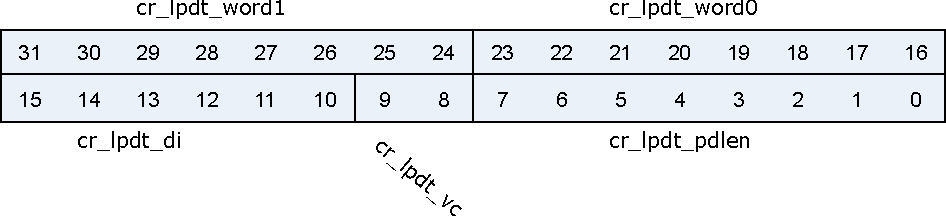
\includegraphics{dsi_dsi_lpdt_tx_config.pdf}
\end{figure}

\regdes{31:24&cr\_lpdt\_word1&r/w&8'h0&LPDT TX word 1\\\hline
23:16&cr\_lpdt\_word0&r/w&8'h0&LPDT TX word 0\\\hline
15:10&cr\_lpdt\_di&r/w&6'h0&LPDT TX data identifier\\\hline
9:8&cr\_lpdt\_vc&r/w&2'h0&LPDT TX virtual channel\\\hline
7:0&cr\_lpdt\_pdlen&r/w&8'd0&LPDT TX packet data length (exclude packet header \& footer) (unit: byte)\\\hline

}
\subsection{dsi\_hstx\_config}
\label{dsi-dsi-hstx-config}
Address:0x3001a10c
 \begin{figure}[H]
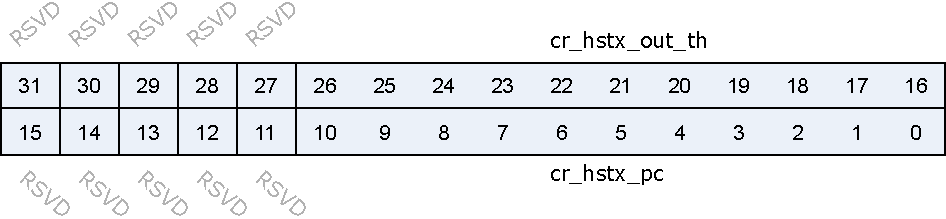
\includegraphics{dsi_dsi_hstx_config.pdf}
\end{figure}

\regdes{31:27&RSVD& & & \\\hline
26:16&cr\_hstx\_out\_th&r/w&11'd840&Line buffer threshold for controller to start transmitting each line (unit: pixel) \par Formula: th = ceil( W * (1 - Fdp*BPP/Fhs/Ln) ) \par th: cr\_hstx\_out\_th \par W: Frame width \par Fdp: Display (dp\_dvp\_tsrc) clock rate \par Fhs: DSI byte clock rate (dsi\_bit\_clk/8 or mipipll\_clk/8) \par BPP: Byte-per-pixel (equals 3 for RGB888 \& RGB666; equals 2 for RGB565 \& YUV422\_8) \par Ln: DSI lane number (controlled by cr\_lane\_num) \par Note: The minimum value is 6 for synchronization concern (Set to 6 if the formula result is negative or less than 6)
\\\hline
15:11&RSVD& & & \\\hline
10:0&cr\_hstx\_pc&r/w&11'd1280&Pixel count of each line (frame width) (unit:pixel) \par Note: Pixel count should not exceed 1280 (720p) and should be a multiple of 4
\\\hline

}
\subsection{dsi\_int\_status}
\label{dsi-dsi-int-status}
Address:0x3001a110
 \begin{figure}[H]
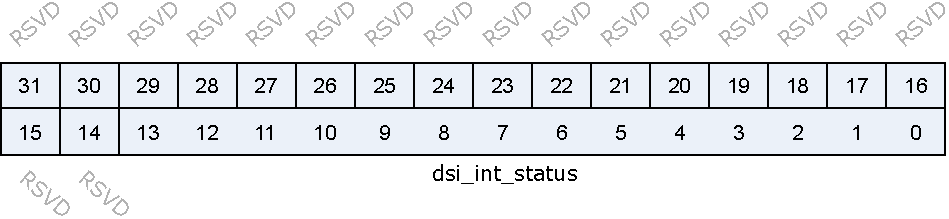
\includegraphics{dsi_dsi_int_status.pdf}
\end{figure}

\regdes{31:14&RSVD& & & \\\hline
13:0&dsi\_int\_status&r&14'h0&[13]: FIFO Error (check 0x60[7:4] for detail) \par [12]: Pixel Count Too Large Error \par [11]: Pixel Count Too Small Error \par [10]: Buffer Underrun Error \par [9]: Buffer Overrun Error \par  \par [8]: RX LPDT FIFO ready \par [7]: TX LPDT FIFO ready \par [6:3]: RX Trigger Command \par [2]: RX ULPS Command \par [1]: RX LPDT End \par [0]: TX Escape Command End
\\\hline

}
\subsection{dsi\_int\_mask}
\label{dsi-dsi-int-mask}
Address:0x3001a114
 \begin{figure}[H]
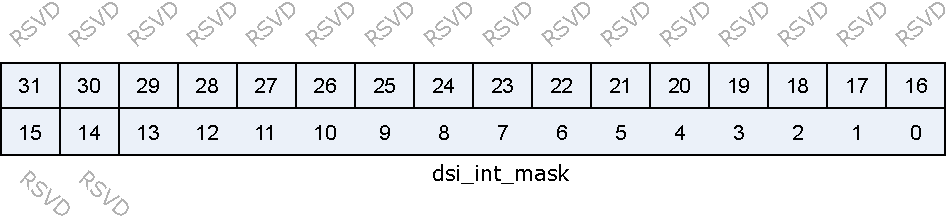
\includegraphics{dsi_dsi_int_mask.pdf}
\end{figure}

\regdes{31:14&RSVD& & & \\\hline
13:0&dsi\_int\_mask&r/w&14'h3FFF&[13]: FIFO Error (check 0x60[7:4] for detail) \par [12]: Pixel Count Too Large Error \par [11]: Pixel Count Too Small Error \par [10]: Buffer Underrun Error \par [9]: Buffer Overrun Error \par  \par [8]: RX LPDT FIFO ready \par [7]: TX LPDT FIFO ready \par [6:3]: RX Trigger Command \par [2]: RX ULPS Command \par [1]: RX LPDT End \par [0]: TX Escape Command End
\\\hline

}
\subsection{dsi\_int\_clear}
\label{dsi-dsi-int-clear}
Address:0x3001a118
 \begin{figure}[H]
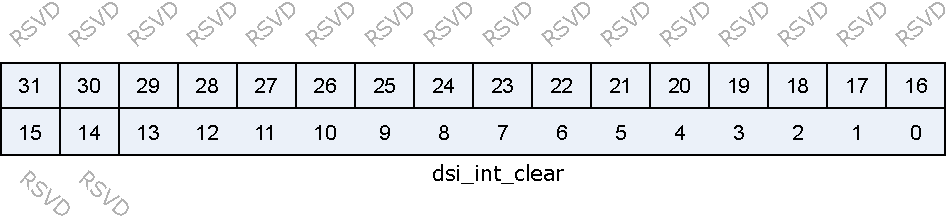
\includegraphics{dsi_dsi_int_clear.pdf}
\end{figure}

\regdes{31:14&RSVD& & & \\\hline
13:0&dsi\_int\_clear&w1p&14'h0&[13]: FIFO Error (check 0x60[7:4] for detail) \par [12]: Pixel Count Too Large Error \par [11]: Pixel Count Too Small Error \par [10]: Buffer Underrun Error \par [9]: Buffer Overrun Error \par  \par [8]: RX LPDT FIFO ready \par [7]: TX LPDT FIFO ready \par [6:3]: RX Trigger Command \par [2]: RX ULPS Command \par [1]: RX LPDT End \par [0]: TX Escape Command End
\\\hline

}
\subsection{dsi\_int\_enable}
\label{dsi-dsi-int-enable}
Address:0x3001a11c
 \begin{figure}[H]
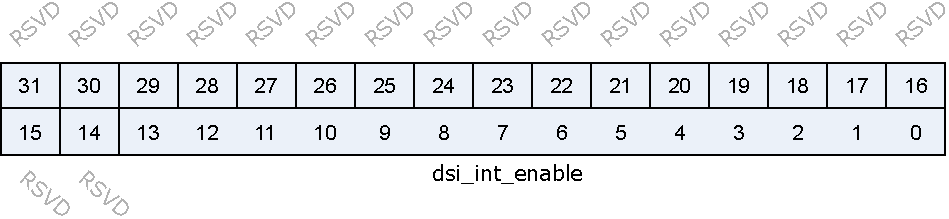
\includegraphics{dsi_dsi_int_enable.pdf}
\end{figure}

\regdes{31:14&RSVD& & & \\\hline
13:0&dsi\_int\_enable&r/w&14'h3FFF&[13]: FIFO Error (check 0x60[7:4] for detail) \par [12]: Pixel Count Too Large Error \par [11]: Pixel Count Too Small Error \par [10]: Buffer Underrun Error \par [9]: Buffer Overrun Error \par  \par [8]: RX LPDT FIFO ready \par [7]: TX LPDT FIFO ready \par [6:3]: RX Trigger Command \par [2]: RX ULPS Command \par [1]: RX LPDT End \par [0]: TX Escape Command End
\\\hline

}
\subsection{dsi\_fifo\_config\_0}
\label{dsi-dsi-fifo-config-0}
Address:0x3001a160
 \begin{figure}[H]
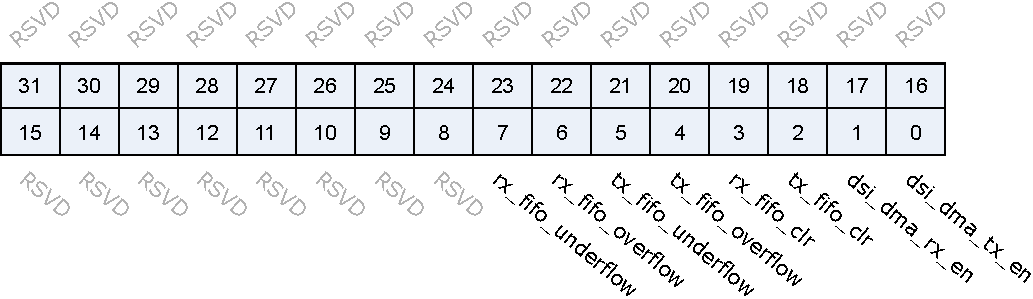
\includegraphics{dsi_dsi_fifo_config_0.pdf}
\end{figure}

\regdes{31:8&RSVD& & & \\\hline
7&rx\_fifo\_underflow&r&1'b0&Underflow flag of RX FIFO, can be cleared by rx\_fifo\_clr\\\hline
6&rx\_fifo\_overflow&r&1'b0&Overflow flag of RX FIFO, can be cleared by rx\_fifo\_clr\\\hline
5&tx\_fifo\_underflow&r&1'b0&Underflow flag of TX FIFO, can be cleared by tx\_fifo\_clr\\\hline
4&tx\_fifo\_overflow&r&1'b0&Overflow flag of TX FIFO, can be cleared by tx\_fifo\_clr\\\hline
3&rx\_fifo\_clr&w1p&1'b0&Clear signal of RX FIFO\\\hline
2&tx\_fifo\_clr&w1p&1'b0&Clear signal of TX FIFO\\\hline
1&dsi\_dma\_rx\_en&r/w&1'b0&Enable signal of dma\_rx\_req/ack interface\\\hline
0&dsi\_dma\_tx\_en&r/w&1'b0&Enable signal of dma\_tx\_req/ack interface\\\hline

}
\subsection{dsi\_fifo\_config\_1}
\label{dsi-dsi-fifo-config-1}
Address:0x3001a164
 \begin{figure}[H]
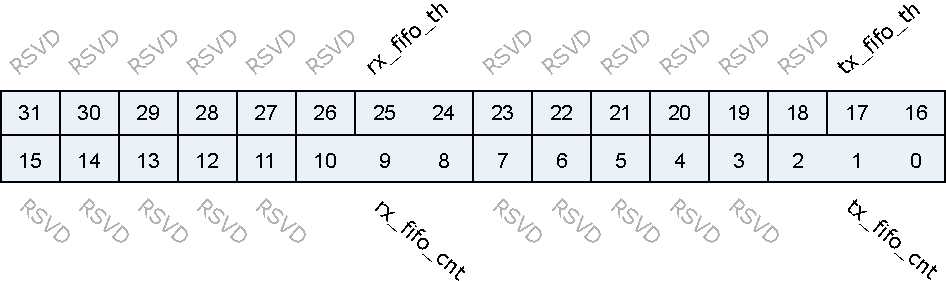
\includegraphics{dsi_dsi_fifo_config_1.pdf}
\end{figure}

\regdes{31:26&RSVD& & & \\\hline
25:24&rx\_fifo\_th&r/w&2'd0&RX FIFO threshold, dma\_rx\_req will not be asserted if tx\_fifo\_cnt is less than this value\\\hline
23:18&RSVD& & & \\\hline
17:16&tx\_fifo\_th&r/w&2'd0&TX FIFO threshold, dma\_tx\_req will not be asserted if tx\_fifo\_cnt is less than this value\\\hline
15:11&RSVD& & & \\\hline
10:8&rx\_fifo\_cnt&r&3'd0&RX FIFO available count\\\hline
7:3&RSVD& & & \\\hline
2:0&tx\_fifo\_cnt&r&3'd4&TX FIFO available count\\\hline

}
\subsection{dsi\_fifo\_wdata}
\label{dsi-dsi-fifo-wdata}
Address:0x3001a168
 \begin{figure}[H]
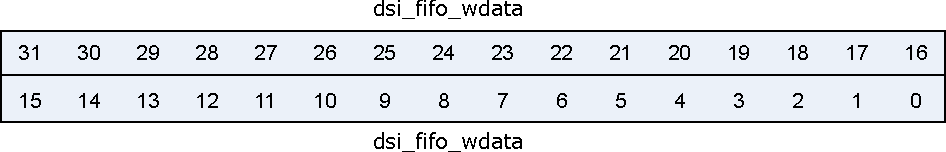
\includegraphics{dsi_dsi_fifo_wdata.pdf}
\end{figure}

\regdes{31:0&dsi\_fifo\_wdata&w&x&\\\hline

}
\subsection{dsi\_fifo\_rdata}
\label{dsi-dsi-fifo-rdata}
Address:0x3001a16c
 \begin{figure}[H]
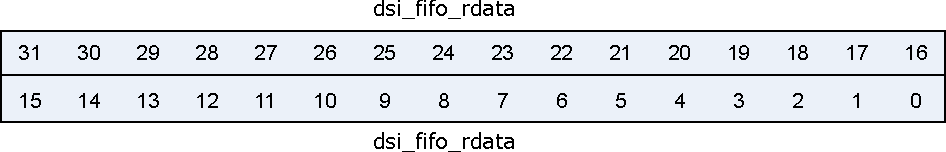
\includegraphics{dsi_dsi_fifo_rdata.pdf}
\end{figure}

\regdes{31:0&dsi\_fifo\_rdata&r&32'h0&\\\hline

}
\subsection{dphy\_config\_0}
\label{dsi-dphy-config-0}
Address:0x3001a180
 \begin{figure}[H]
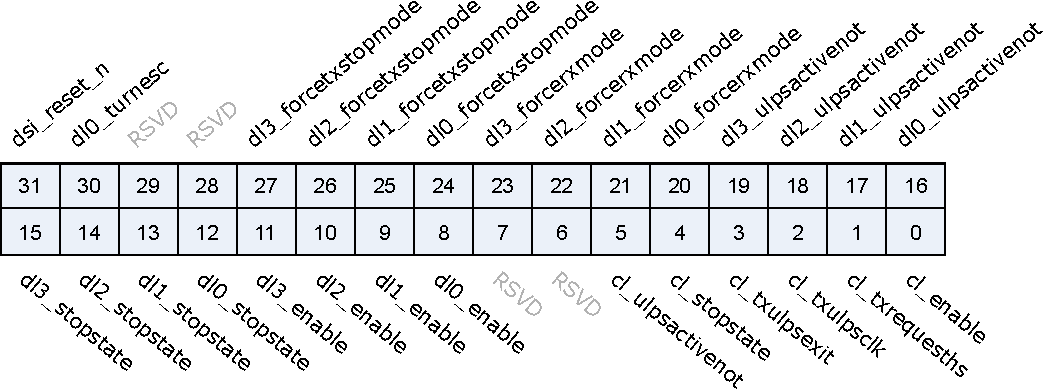
\includegraphics{dsi_dphy_config_0.pdf}
\end{figure}

\regdes{31&dsi\_reset\_n&r/w&1'b0&MIPI DSI D-PHY reset pin\\\hline
30&dl0\_turnesc&w1p&1'b0&Data lane0 Bus Turnaround\\\hline
29:28&RSVD& & & \\\hline
27&dl3\_forcetxstopmode&r/w&1'b0&Force Lane3 to Generate Stop State\\\hline
26&dl2\_forcetxstopmode&r/w&1'b0&Force Lane2 to Generate Stop State\\\hline
25&dl1\_forcetxstopmode&r/w&1'b0&Force Lane1 to Generate Stop State\\\hline
24&dl0\_forcetxstopmode&r/w&1'b0&Force Lane0 to Generate Stop State\\\hline
23&dl3\_forcerxmode&r/w&1'b0&Enables the reverse escape LP receiver. Lane3 immediately transitions to receive mode.\\\hline
22&dl2\_forcerxmode&r/w&1'b0&Enables the reverse escape LP receiver. Lane2 immediately transitions to receive mode.\\\hline
21&dl1\_forcerxmode&r/w&1'b0&Enables the reverse escape LP receiver. Lane1 immediately transitions to receive mode.\\\hline
20&dl0\_forcerxmode&r/w&1'b0&Enables the reverse escape LP receiver. Lane0 immediately transitions to receive mode.\\\hline
19&dl3\_ulpsactivenot&r&1'b1&Data lane3 is NOT in the ULP state\\\hline
18&dl2\_ulpsactivenot&r&1'b1&Data lane2 is NOT in the ULP state\\\hline
17&dl1\_ulpsactivenot&r&1'b1&Data lane1 is NOT in the ULP state\\\hline
16&dl0\_ulpsactivenot&r&1'b1&Data lane0 is NOT in the ULP state\\\hline
15&dl3\_stopstate&r&1'b1&Data lane3 is in Stop state\\\hline
14&dl2\_stopstate&r&1'b1&Data lane2 is in Stop state\\\hline
13&dl1\_stopstate&r&1'b1&Data lane1 is in Stop state\\\hline
12&dl0\_stopstate&r&1'b1&Data lane0 is in Stop state\\\hline
11&dl3\_enable&r/w&1'b0&Data lane3 enable\\\hline
10&dl2\_enable&r/w&1'b0&Data lane2 enable\\\hline
9&dl1\_enable&r/w&1'b0&Data lane1 enable\\\hline
8&dl0\_enable&r/w&1'b0&Data lane0 enable\\\hline
7:6&RSVD& & & \\\hline
5&cl\_ulpsactivenot&r&1'b1&Clock lane is NOT in the ULP state\\\hline
4&cl\_stopstate&r&1'b1&Clock lane is in Stop state\\\hline
3&cl\_txulpsexit&w1p&1'b0&Clock lane Transmit ULP Exit Sequence\\\hline
2&cl\_txulpsclk&r/w&1'b0&Clock lane Transmit Ultra-Low Power State\\\hline
1&cl\_txrequesths&r/w&1'b0&Clock lane High-Speed Transmit Request\\\hline
0&cl\_enable&r/w&1'b0&Clock lane enable\\\hline

}
\subsection{dphy\_config\_1}
\label{dsi-dphy-config-1}
Address:0x3001a184
 \begin{figure}[H]
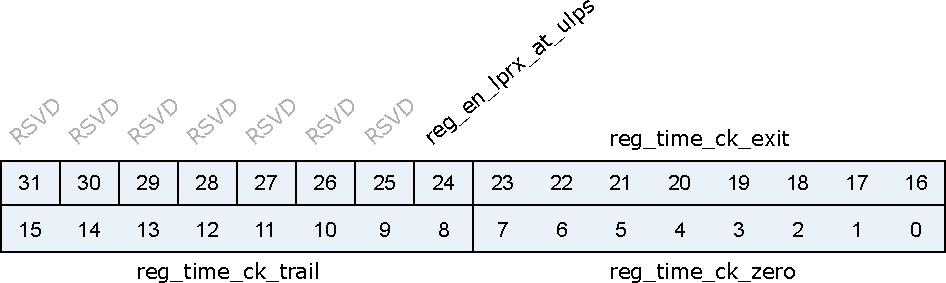
\includegraphics{dsi_dphy_config_1.pdf}
\end{figure}

\regdes{31:25&RSVD& & & \\\hline
24&reg\_en\_lprx\_at\_ulps&r/w&1'b0&MIPI DSI D-PHY control register - reg\_en\_lprx\_at\_ulps\\\hline
23:16&reg\_time\_ck\_exit&r/w&8'h5&MIPI DSI D-PHY control register - reg\_time\_ck\_exit (tx\_clk\_esc) txclkesc: 40M, datarate: 800Mbps\\\hline
15:8&reg\_time\_ck\_trail&r/w&8'h3&MIPI DSI D-PHY control register - reg\_time\_ck\_trail (tx\_clk\_esc)\\\hline
7:0&reg\_time\_ck\_zero&r/w&8'hF&MIPI DSI D-PHY control register - reg\_time\_ck\_zero (tx\_clk\_esc)\\\hline

}
\subsection{dphy\_config\_2}
\label{dsi-dphy-config-2}
Address:0x3001a188
 \begin{figure}[H]
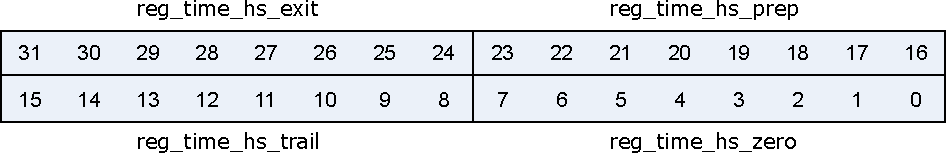
\includegraphics{dsi_dphy_config_2.pdf}
\end{figure}

\regdes{31:24&reg\_time\_hs\_exit&r/w&8'h5&MIPI DSI D-PHY control register - reg\_time\_hs\_exit (tx\_clk\_esc)\\\hline
23:16&reg\_time\_hs\_prep&r/w&8'h2&MIPI DSI D-PHY control register - reg\_time\_hs\_prep (tx\_clk\_esc)\\\hline
15:8&reg\_time\_hs\_trail&r/w&8'h3&MIPI DSI D-PHY control register - reg\_time\_hs\_trail (tx\_clk\_esc)\\\hline
7:0&reg\_time\_hs\_zero&r/w&8'h5&MIPI DSI D-PHY control register - reg\_time\_hs\_zero (tx\_clk\_esc)\\\hline

}
\subsection{dphy\_config\_3}
\label{dsi-dphy-config-3}
Address:0x3001a18c
 \begin{figure}[H]
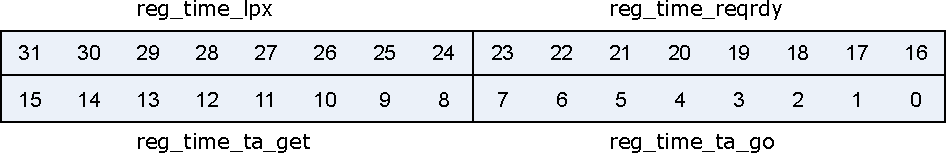
\includegraphics{dsi_dphy_config_3.pdf}
\end{figure}

\regdes{31:24&reg\_time\_lpx&r/w&8'h3&MIPI DSI D-PHY control register - reg\_time\_lpx (tx\_clk\_esc)\\\hline
23:16&reg\_time\_reqrdy&r/w&8'h0&MIPI DSI D-PHY control register - reg\_time\_reqrdy\\\hline
15:8&reg\_time\_ta\_get&r/w&8'hF&MIPI DSI D-PHY control register - reg\_time\_ta\_get (tx\_clk\_esc)\\\hline
7:0&reg\_time\_ta\_go&r/w&8'hC&MIPI DSI D-PHY control register - reg\_time\_ta\_go (tx\_clk\_esc)\\\hline

}
\subsection{dphy\_config\_4}
\label{dsi-dphy-config-4}
Address:0x3001a190
 \begin{figure}[H]
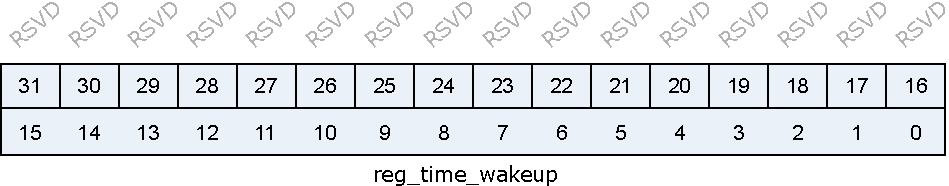
\includegraphics{dsi_dphy_config_4.pdf}
\end{figure}

\regdes{31:16&RSVD& & & \\\hline
15:0&reg\_time\_wakeup&r/w&16'h9C41&MIPI DSI D-PHY control register - reg\_time\_wakeup (tx\_clk\_esc)\\\hline

}
\subsection{dphy\_config\_5}
\label{dsi-dphy-config-5}
Address:0x3001a194
 \begin{figure}[H]
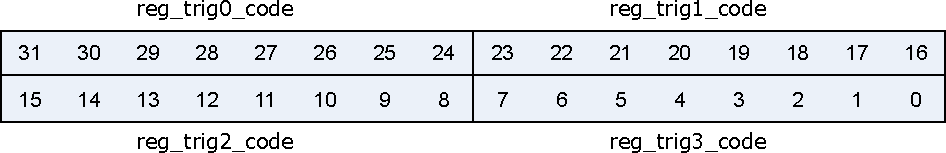
\includegraphics{dsi_dphy_config_5.pdf}
\end{figure}

\regdes{31:24&reg\_trig0\_code&r/w&8'b0100\_0110&MIPI DSI D-PHY control register - reg\_trig0\_code\\\hline
23:16&reg\_trig1\_code&r/w&8'b1011\_1010&MIPI DSI D-PHY control register - reg\_trig1\_code\\\hline
15:8&reg\_trig2\_code&r/w&8'b1000\_0100&MIPI DSI D-PHY control register - reg\_trig2\_code\\\hline
7:0&reg\_trig3\_code&r/w&8'b0000\_0101&MIPI DSI D-PHY control register - reg\_trig3\_code\\\hline

}
\subsection{dphy\_config\_6}
\label{dsi-dphy-config-6}
Address:0x3001a198
 \begin{figure}[H]
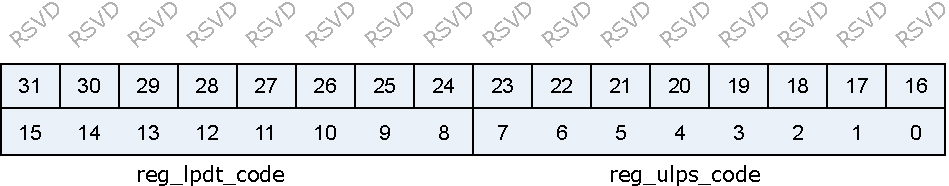
\includegraphics{dsi_dphy_config_6.pdf}
\end{figure}

\regdes{31:16&RSVD& & & \\\hline
15:8&reg\_lpdt\_code&r/w&8'b1000\_0111&MIPI DSI D-PHY control register - reg\_lpdt\_code\\\hline
7:0&reg\_ulps\_code&r/w&8'b0111\_1000&MIPI DSI D-PHY control register - reg\_ulps\_code\\\hline

}
\subsection{dphy\_config\_7}
\label{dsi-dphy-config-7}
Address:0x3001a19c
 \begin{figure}[H]
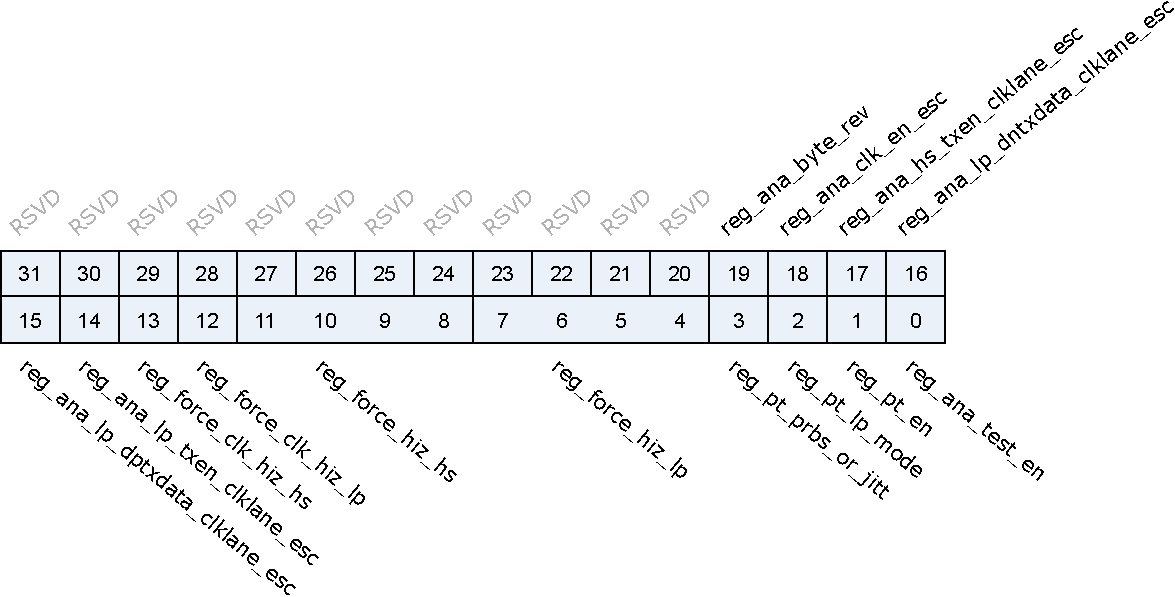
\includegraphics{dsi_dphy_config_7.pdf}
\end{figure}

\regdes{31:20&RSVD& & & \\\hline
19&reg\_ana\_byte\_rev&r/w&1'b0&MIPI DSI D-PHY control register - reg\_ana\_byte\_rev\\\hline
18&reg\_ana\_clk\_en\_esc&r/w&1'b0&MIPI DSI D-PHY control register - reg\_ana\_clk\_en\_esc\\\hline
17&reg\_ana\_hs\_txen\_clklane\_esc&r/w&1'b0&MIPI DSI D-PHY control register - reg\_ana\_hs\_txen\_clklane\_esc\\\hline
16&reg\_ana\_lp\_dntxdata\_clklane\_esc&r/w&1'b0&MIPI DSI D-PHY control register - reg\_ana\_lp\_dntxdata\_clklane\_esc\\\hline
15&reg\_ana\_lp\_dptxdata\_clklane\_esc&r/w&1'b0&MIPI DSI D-PHY control register - reg\_ana\_lp\_dptxdata\_clklane\_esc\\\hline
14&reg\_ana\_lp\_txen\_clklane\_esc&r/w&1'b0&MIPI DSI D-PHY control register - reg\_ana\_lp\_txen\_clklane\_esc\\\hline
13&reg\_force\_clk\_hiz\_hs&r/w&1'b0&MIPI DSI D-PHY control register - reg\_force\_clk\_hiz\_hs\\\hline
12&reg\_force\_clk\_hiz\_lp&r/w&1'b0&MIPI DSI D-PHY control register - reg\_force\_clk\_hiz\_lp\\\hline
11:8&reg\_force\_hiz\_hs&r/w&4'h0&MIPI DSI D-PHY control register - reg\_force\_hiz\_hs\\\hline
7:4&reg\_force\_hiz\_lp&r/w&4'h0&MIPI DSI D-PHY control register - reg\_force\_hiz\_lp\\\hline
3&reg\_pt\_prbs\_or\_jitt&r/w&1'b0&MIPI DSI D-PHY control register - reg\_pt\_prbs\_or\_jitt\\\hline
2&reg\_pt\_lp\_mode&r/w&1'b0&MIPI DSI D-PHY control register - reg\_pt\_lp\_mode\\\hline
1&reg\_pt\_en&r/w&1'b0&MIPI DSI D-PHY control register - reg\_pt\_en\\\hline
0&reg\_ana\_test\_en&r/w&1'b0&MIPI DSI D-PHY control register - reg\_ana\_test\_en\\\hline

}
\subsection{dphy\_config\_8}
\label{dsi-dphy-config-8}
Address:0x3001a1a0
 \begin{figure}[H]
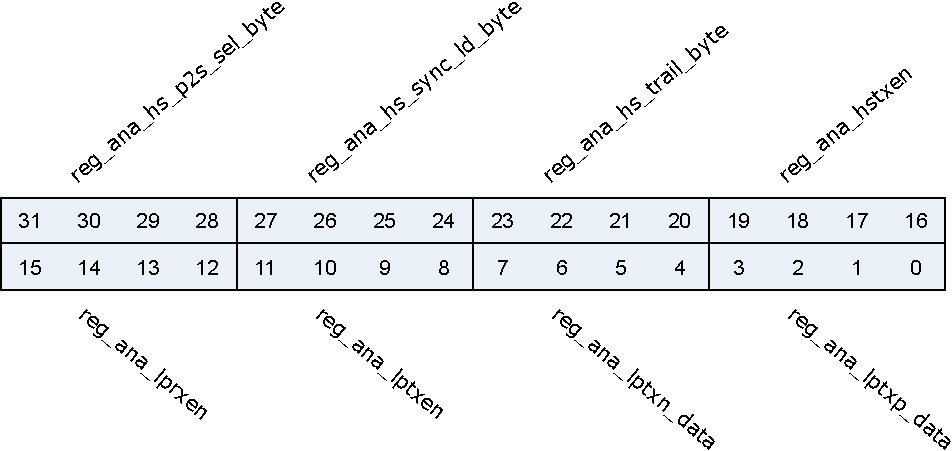
\includegraphics{dsi_dphy_config_8.pdf}
\end{figure}

\regdes{31:28&reg\_ana\_hs\_p2s\_sel\_byte&r/w&4'h0&MIPI DSI D-PHY control register - reg\_ana\_hs\_p2s\_sel\_byte\\\hline
27:24&reg\_ana\_hs\_sync\_ld\_byte&r/w&4'h0&MIPI DSI D-PHY control register - reg\_ana\_hs\_sync\_ld\_byte\\\hline
23:20&reg\_ana\_hs\_trail\_byte&r/w&4'h0&MIPI DSI D-PHY control register - reg\_ana\_hs\_trail\_byte\\\hline
19:16&reg\_ana\_hstxen&r/w&4'h0&MIPI DSI D-PHY control register - reg\_ana\_hstxen\\\hline
15:12&reg\_ana\_lprxen&r/w&4'h0&MIPI DSI D-PHY control register - reg\_ana\_lprxen\\\hline
11:8&reg\_ana\_lptxen&r/w&4'h0&MIPI DSI D-PHY control register - reg\_ana\_lptxen\\\hline
7:4&reg\_ana\_lptxn\_data&r/w&4'h0&MIPI DSI D-PHY control register - reg\_ana\_lptxn\_data\\\hline
3:0&reg\_ana\_lptxp\_data&r/w&4'h0&MIPI DSI D-PHY control register - reg\_ana\_lptxp\_data\\\hline

}
\subsection{dphy\_config\_9}
\label{dsi-dphy-config-9}
Address:0x3001a1a4
 \begin{figure}[H]
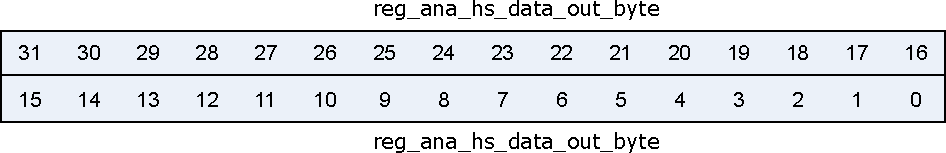
\includegraphics{dsi_dphy_config_9.pdf}
\end{figure}

\regdes{31:0&reg\_ana\_hs\_data\_out\_byte&r/w&32'h0&MIPI DSI D-PHY control register - reg\_ana\_hs\_data\_out\_byte\\\hline

}
\subsection{dphy\_config\_10}
\label{dsi-dphy-config-10}
Address:0x3001a1a8
 \begin{figure}[H]
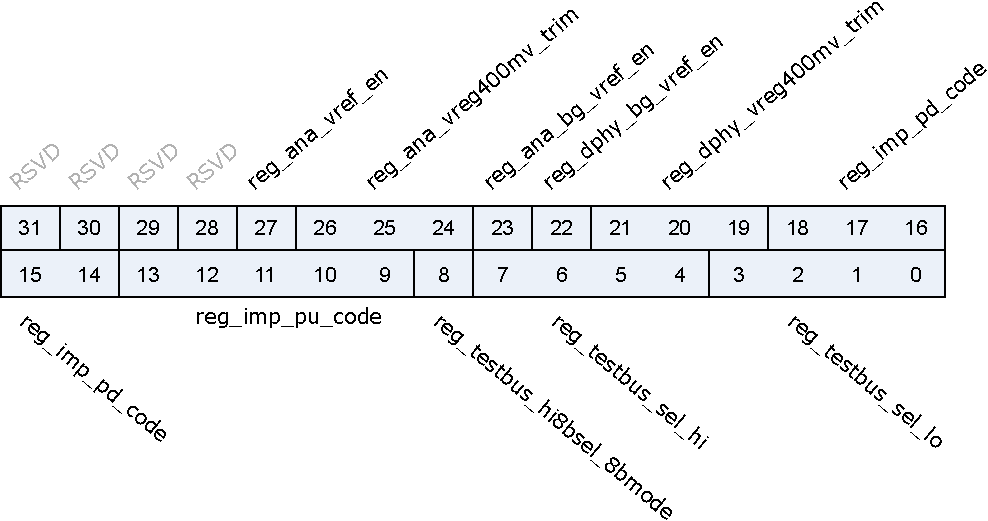
\includegraphics{dsi_dphy_config_10.pdf}
\end{figure}

\regdes{31:28&RSVD& & & \\\hline
27&reg\_ana\_vref\_en&r/w&1'b0&MIPI DSI D-PHY control register - reg\_ana\_vref\_en\\\hline
26:24&reg\_ana\_vreg400mv\_trim&r/w&3'h0&MIPI DSI D-PHY control register - reg\_ana\_vreg400mv\_trim\\\hline
23&reg\_ana\_bg\_vref\_en&r/w&1'b0&MIPI DSI D-PHY control register - reg\_ana\_bg\_vref\_en\\\hline
22&reg\_dphy\_bg\_vref\_en&r/w&1'b0&MIPI DSI D-PHY control register - reg\_dphy\_bg\_vref\_en\\\hline
21:19&reg\_dphy\_vreg400mv\_trim&r/w&3'h0&MIPI DSI D-PHY control register - reg\_dphy\_vreg400mv\_trim\\\hline
18:14&reg\_imp\_pd\_code&r/w&5'h9&MIPI DSI D-PHY control register - reg\_imp\_pd\_code\\\hline
13:9&reg\_imp\_pu\_code&r/w&5'h8&MIPI DSI D-PHY control register - reg\_imp\_pu\_code\\\hline
8&reg\_testbus\_hi8bsel\_8bmode&r/w&1'b0&MIPI DSI D-PHY control register - reg\_testbus\_hi8bsel\_8bmode\\\hline
7:4&reg\_testbus\_sel\_hi&r/w&4'h0&MIPI DSI D-PHY control register - reg\_testbus\_sel\_hi\\\hline
3:0&reg\_testbus\_sel\_lo&r/w&4'h0&MIPI DSI D-PHY control register - reg\_testbus\_sel\_lo\\\hline

}
\subsection{dphy\_config\_11}
\label{dsi-dphy-config-11}
Address:0x3001a1ac
 \begin{figure}[H]
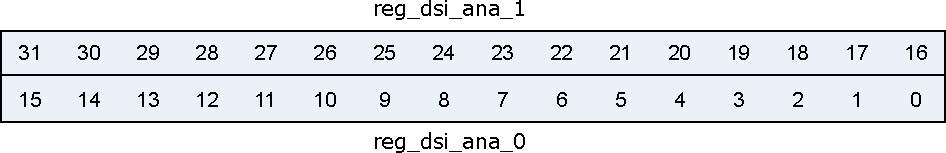
\includegraphics{dsi_dphy_config_11.pdf}
\end{figure}

\regdes{31:16&reg\_dsi\_ana\_1&r/w&16'h0&MIPI DSI D-PHY control register - reg\_dsi\_ana\_1\\\hline
15:0&reg\_dsi\_ana\_0&r/w&16'hc14&MIPI DSI D-PHY control register - reg\_dsi\_ana\_0\\\hline

}
\subsection{dphy\_config\_12}
\label{dsi-dphy-config-12}
Address:0x3001a1b0
 \begin{figure}[H]
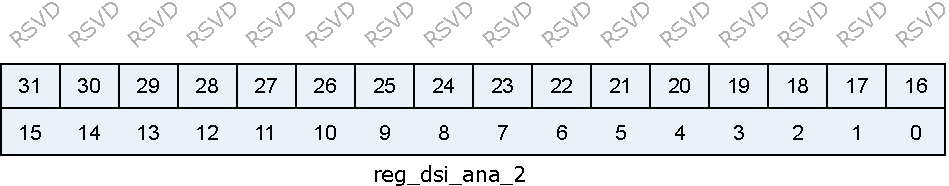
\includegraphics{dsi_dphy_config_12.pdf}
\end{figure}

\regdes{31:16&RSVD& & & \\\hline
15:0&reg\_dsi\_ana\_2&r/w&16'h0&MIPI DSI D-PHY control register - reg\_dsi\_ana\_2\\\hline

}
\subsection{dphy\_config\_13}
\label{dsi-dphy-config-13}
Address:0x3001a1b4
 \begin{figure}[H]
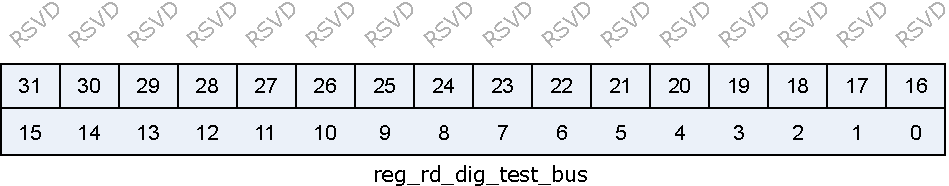
\includegraphics{dsi_dphy_config_13.pdf}
\end{figure}

\regdes{31:16&RSVD& & & \\\hline
15:0&reg\_rd\_dig\_test\_bus&r&16'h0&MIPI DSI D-PHY control register - reg\_rd\_dig\_test\_bus\\\hline

}
\subsection{dphy\_config\_14}
\label{dsi-dphy-config-14}
Address:0x3001a1b8
 \begin{figure}[H]
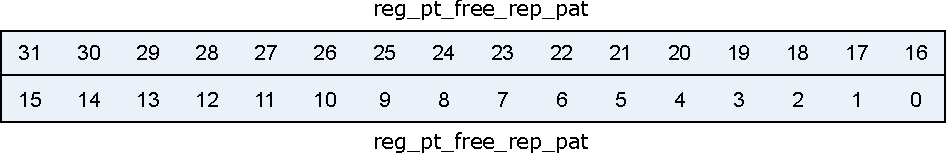
\includegraphics{dsi_dphy_config_14.pdf}
\end{figure}

\regdes{31:0&reg\_pt\_free\_rep\_pat&r/w&32'h87654321&MIPI DSI D-PHY control register - reg\_pt\_free\_rep\_pat\\\hline

}
\subsection{dphy\_config\_15}
\label{dsi-dphy-config-15}
Address:0x3001a1bc
 \begin{figure}[H]
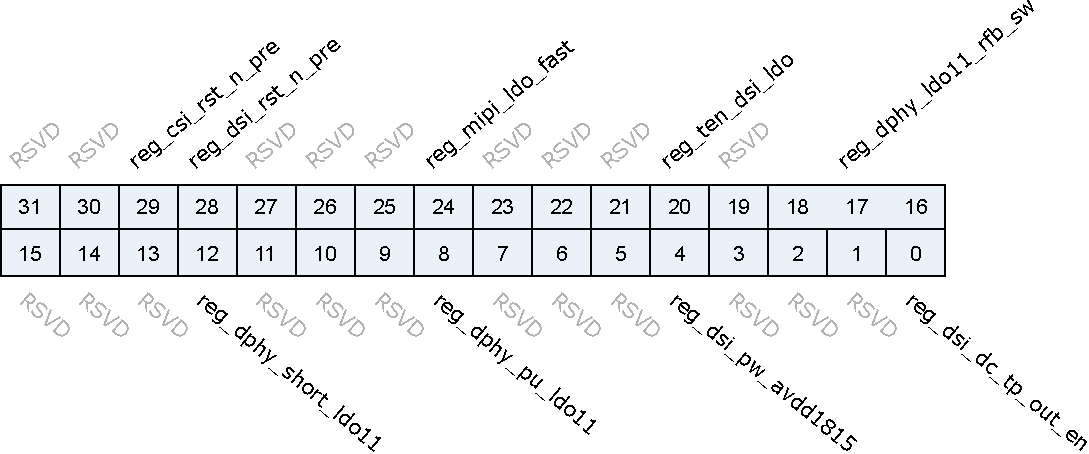
\includegraphics{dsi_dphy_config_15.pdf}
\end{figure}

\regdes{31:30&RSVD& & & \\\hline
29&reg\_csi\_rst\_n\_pre&r/w&1'b0&Note: reg\_csi\_rst\_n\_pre should be released at least 2 us BEFORE releasing csi\_reset\_n\\\hline
28&reg\_dsi\_rst\_n\_pre&r/w&1'b0&Note: reg\_dsi\_rst\_n\_pre should be released at least 2 us BEFORE releasing dsi\_reset\_n\\\hline
27:25&RSVD& & & \\\hline
24&reg\_mipi\_ldo\_fast&r/w&1'b0&\\\hline
23:21&RSVD& & & \\\hline
20&reg\_ten\_dsi\_ldo&r/w&1'b0&\\\hline
19&RSVD& & & \\\hline
18:16&reg\_dphy\_ldo11\_rfb\_sw&r/w&3'd4&\\\hline
15:13&RSVD& & & \\\hline
12&reg\_dphy\_short\_ldo11&r/w&1'b0&\\\hline
11:9&RSVD& & & \\\hline
8&reg\_dphy\_pu\_ldo11&r/w&1'b1&enable LDO11 for both dsi and csi\\\hline
7:5&RSVD& & & \\\hline
4&reg\_dsi\_pw\_avdd1815&r/w&1'b0&0: power switch on\\\hline
3:1&RSVD& & & \\\hline
0&reg\_dsi\_dc\_tp\_out\_en&r/w&1'b0&\\\hline

}
\subsection{dphy\_config\_16}
\label{dsi-dphy-config-16}
Address:0x3001a1c0
 \begin{figure}[H]
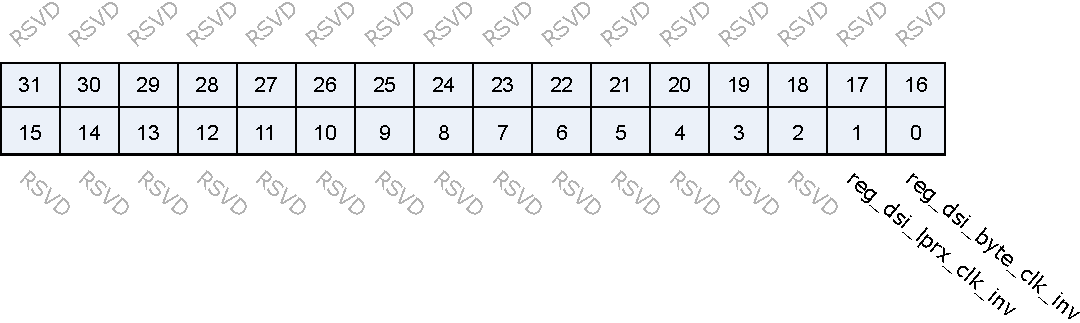
\includegraphics{dsi_dphy_config_16.pdf}
\end{figure}

\regdes{31:2&RSVD& & & \\\hline
1&reg\_dsi\_lprx\_clk\_inv&r/w&1'b0&\\\hline
0&reg\_dsi\_byte\_clk\_inv&r/w&1'b0&\\\hline

}
\subsection{dummy\_reg}
\label{dsi-dummy-reg}
Address:0x3001a1fc
 \begin{figure}[H]
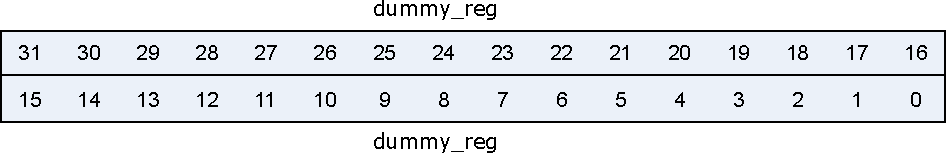
\includegraphics{dsi_dummy_reg.pdf}
\end{figure}

\regdes{31:0&dummy\_reg&r/w&32'h0&Dummy registers\\\hline

}
